% !TeX spellcheck = cs_CZ
%{\tikzset{external/prefix={tikz/FYZII/}}
% \tikzset{external/figure name/.add={ch16_}{}}
%---------------------------------------------------------------------------------------------------
% file fey2ch16.tex
%---------------------------------------------------------------------------------------------------
%====================Kapitola: Indukované proudy ===================================================
\setchaptertoc
\chapter{Indukované proudy}\label{fyz:IIchapXVI}


\section{Motory a generátory}\label{fyz:IIchapXVIsecI}


\section{Transformátory a indukčnosti}\label{fyz:IIchapXVIsecII}

  
\section{Síly působící na indukované proudy}\label{fyz:IIchapXVIsecIII}


\section{Elektrotechnika}\label{fyz:IIchapXVIsecIV}

  \begin{figure}[ht!]  %\ref{fyz:fig311}
    \centering
    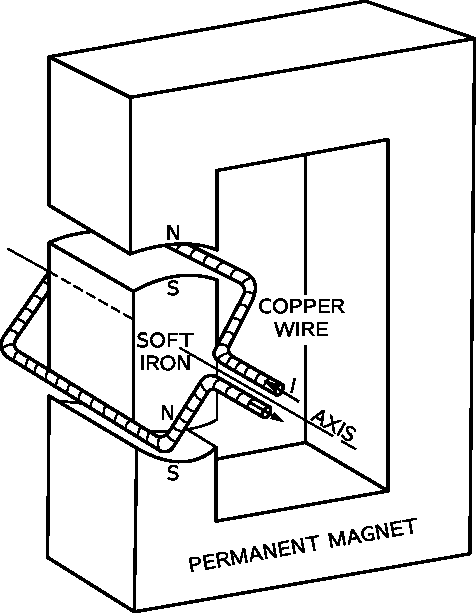
\includegraphics[width=0.8\linewidth]{fyz_fig311.pdf}
    \caption{
             (\cite[s.~148]{Feynman02}).}
    \label{fyz:fig311}
  \end{figure}

  \begin{figure}[ht!]  %\ref{fyz:fig312}
    \centering
    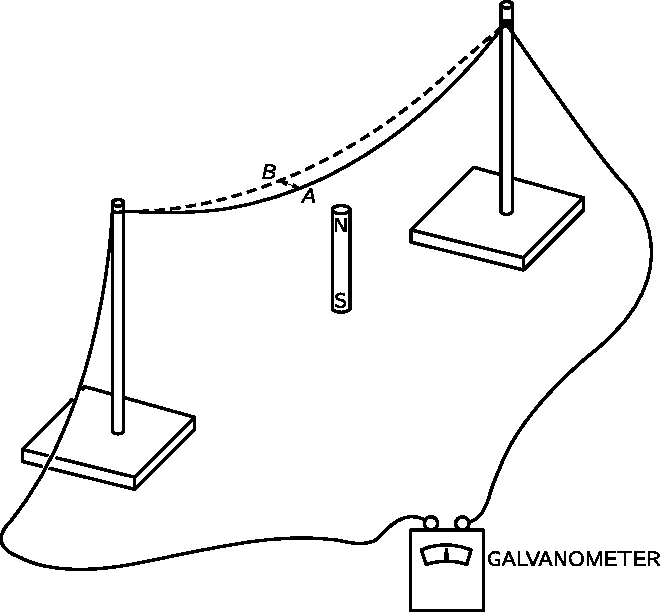
\includegraphics[width=0.8\linewidth]{fyz_fig312.pdf}
    \caption{
             (\cite[s.~148]{Feynman02}).}
    \label{fyz:fig312}
  \end{figure}

  \begin{figure}[ht!]  %\ref{fyz:fig313}
    \centering
    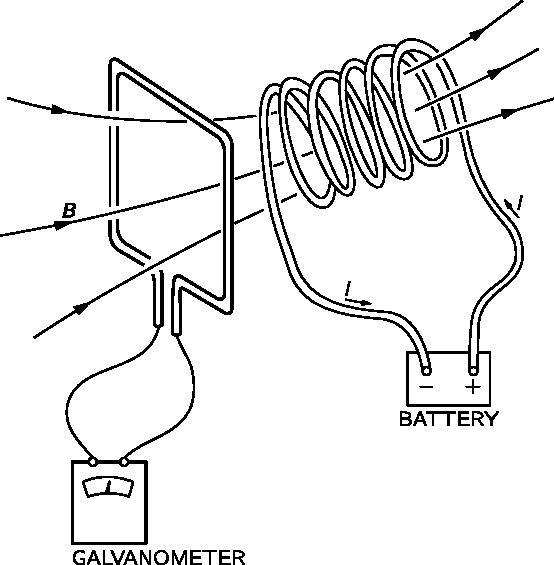
\includegraphics[width=0.8\linewidth]{fyz_fig313.pdf}
    \caption{
             (\cite[s.~148]{Feynman02}).}
    \label{fyz:fig313}
  \end{figure}

  \begin{figure}[ht!]  %\ref{fyz:fig314}
    \centering
    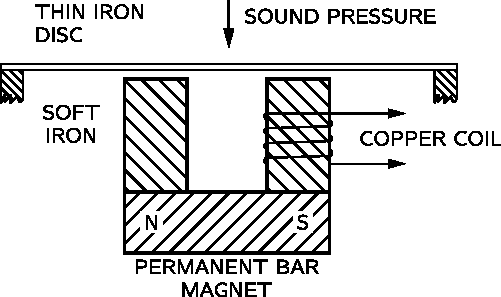
\includegraphics[width=0.8\linewidth]{fyz_fig314.pdf}
    \caption{
             (\cite[s.~148]{Feynman02}).}
    \label{fyz:fig314}
  \end{figure}

  \begin{figure}[ht!]  %\ref{fyz:fig315}
    \centering
    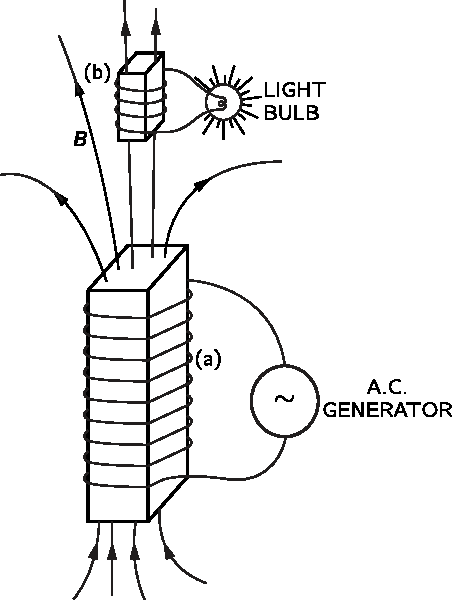
\includegraphics[width=0.8\linewidth]{fyz_fig315.pdf}
    \caption{
             (\cite[s.~148]{Feynman02}).}
    \label{fyz:fig315}
  \end{figure}

  \begin{figure}[ht!]  %\ref{fyz:fig316}
    \centering
    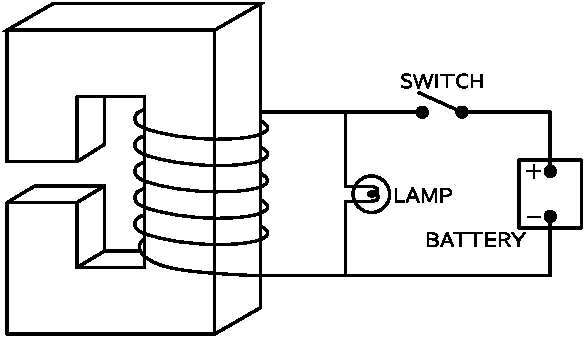
\includegraphics[width=0.8\linewidth]{fyz_fig316.pdf}
    \caption{
             (\cite[s.~148]{Feynman02}).}
    \label{fyz:fig316}
  \end{figure}
  
  \begin{figure}[ht!]  %\ref{fyz:fig317}
    \centering
    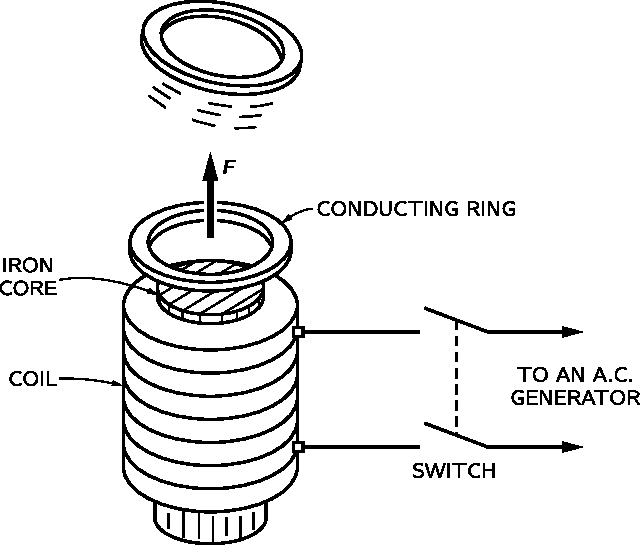
\includegraphics[width=0.8\linewidth]{fyz_fig317.pdf}
    \caption{
             (\cite[s.~148]{Feynman02}).}
    \label{fyz:fig317}
  \end{figure}

  \begin{figure}[ht!]  %\ref{fyz:fig318}
    \centering
    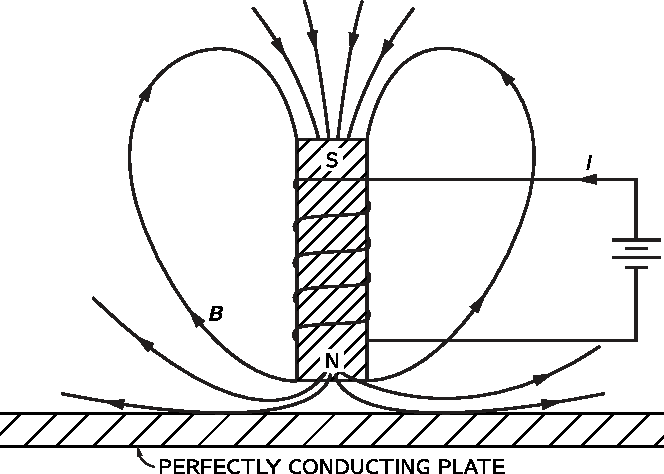
\includegraphics[width=0.8\linewidth]{fyz_fig318.pdf}
    \caption{
             (\cite[s.~148]{Feynman02}).}
    \label{fyz:fig318}
  \end{figure}

  \begin{figure}[ht!]  %\ref{fyz:fig319}
    \centering
    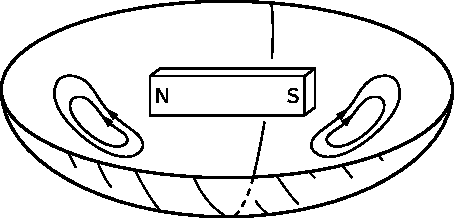
\includegraphics[width=0.8\linewidth]{fyz_fig319.pdf}
    \caption{
             (\cite[s.~148]{Feynman02}).}
    \label{fyz:fig319}
  \end{figure}

  \begin{figure}[ht!]  %\ref{fyz:fig320}
    \centering
    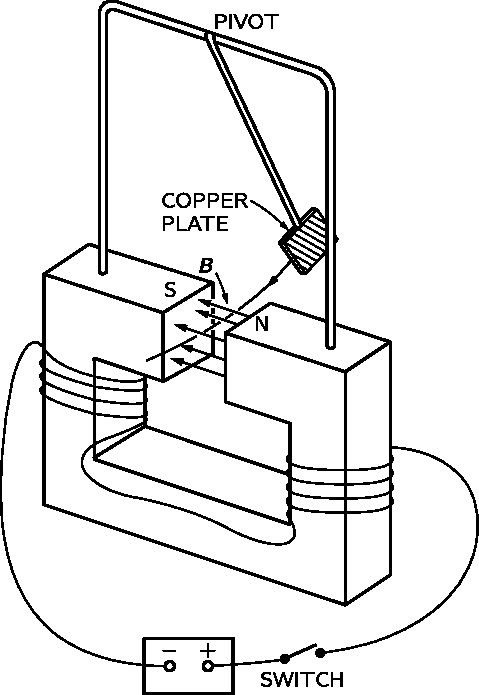
\includegraphics[width=0.8\linewidth]{fyz_fig320.pdf}
    \caption{
             (\cite[s.~148]{Feynman02}).}
    \label{fyz:fig320}
  \end{figure}

  \begin{figure}[ht!]  %\ref{fyz:fig321}
    \centering
    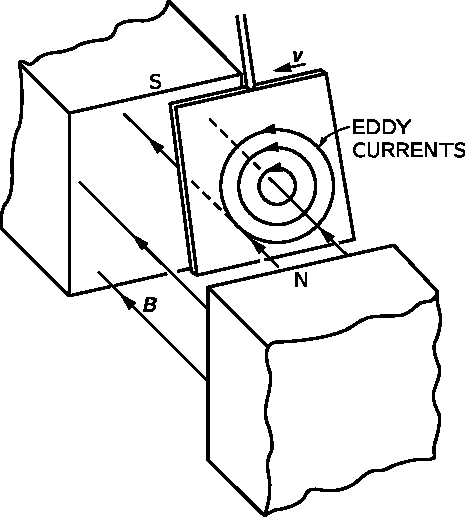
\includegraphics[width=0.8\linewidth]{fyz_fig321.pdf}
    \caption{
             (\cite[s.~148]{Feynman02}).}
    \label{fyz:fig321}
  \end{figure}

  \begin{figure}[ht!]  %\ref{fyz:fig322}
    \centering
    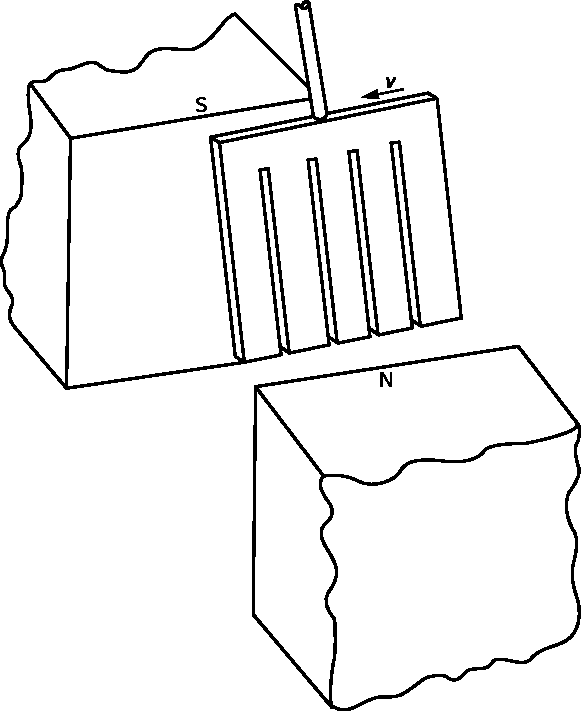
\includegraphics[width=0.8\linewidth]{fyz_fig322.pdf}
    \caption{
             (\cite[s.~148]{Feynman02}).}
    \label{fyz:fig322}
  \end{figure}
  
  \begin{figure}[ht!]  %\ref{fyz:fig323}
    \centering
    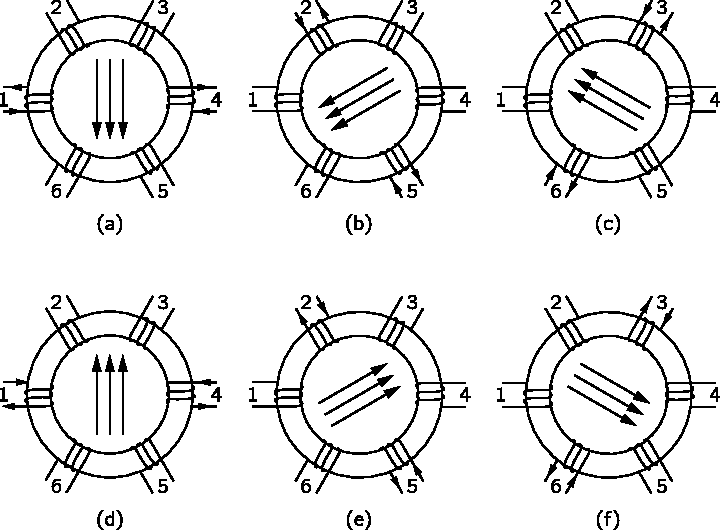
\includegraphics[width=0.8\linewidth]{fyz_fig323.pdf}
    \caption{
             (\cite[s.~148]{Feynman02}).}
    \label{fyz:fig323}
  \end{figure}
  
  \begin{figure}[ht!]  %\ref{fyz:fig324}
    \centering
    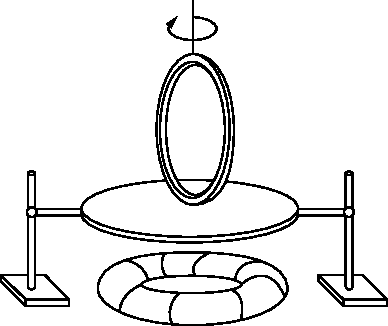
\includegraphics[width=0.8\linewidth]{fyz_fig324.pdf}
    \caption{
             (\cite[s.~148]{Feynman02}).}
    \label{fyz:fig324}
  \end{figure}

  \begin{figure}[hb!]
    \centering
    \subcaptionbox{\label{fyz:fig325a}}{\luafigure[0.45]{fyz_fig325a.pdf}}
    \subcaptionbox{\label{fyz:fig325b}}{\luafigure[0.45]{fyz_fig325b.pdf}}
    \caption{ }
    \label{fyz:fig325}
  \end{figure}

  \todo[inline]{Kapitola fey2ch16 je nedodělaná, obsahuje pouze obrázky}
%} %tikzset
%~~~~~~~~~~~~~~~~~~~~~~~~~~~~~~~~~~~~~~~~~~~~~~~~~~~~~~~~~~~~~~~~~~~~~~~~~~~~~~~~~~~~~~~~~~~~~~~~~~
